\documentclass{article}
\usepackage{graphicx} 
\usepackage{amsmath}
\usepackage{float}
\graphicspath{{images/}}

\title{\textbf{Power Electronics Laboratory
\\Session 3: Isolated DC-DC Converters}}

\author{Team 3 : \\Po Ting Yeh K-9056 \\Beyazit Bilal Ozkaya 341967 \\Braulio Cardenas 342021}
\begin{document}

\maketitle

\section*{Introduction}
This experiment investigates the operation and theoretical characteristics of two isolated DC-DC converters: the flyback converter and the forward converter. In the first part, we analyze the flyback converter in both Continuous Conduction Mode (CCM) and Discontinuous Conduction Mode (DCM). By testing different duty cycles and load steps, we quantitatively verify the output voltage equations and observe the zero-crossing behavior of the magnetizing current. In the second part, we study the forward converter in CCM. We specifically focus on the transformer's reset mechanism, which uses a third winding and a diode to safely discharge the core energy. Finally, by applying an extreme duty cycle step, we mathematically and visually prove the operational limits of the reset circuit and demonstrate how insufficient OFF-time leads to magnetic saturation.

\section*{Part 1:}
\section{Task 1: Continuous Conduction Mode}
\begin{figure}[H]
    \centering
    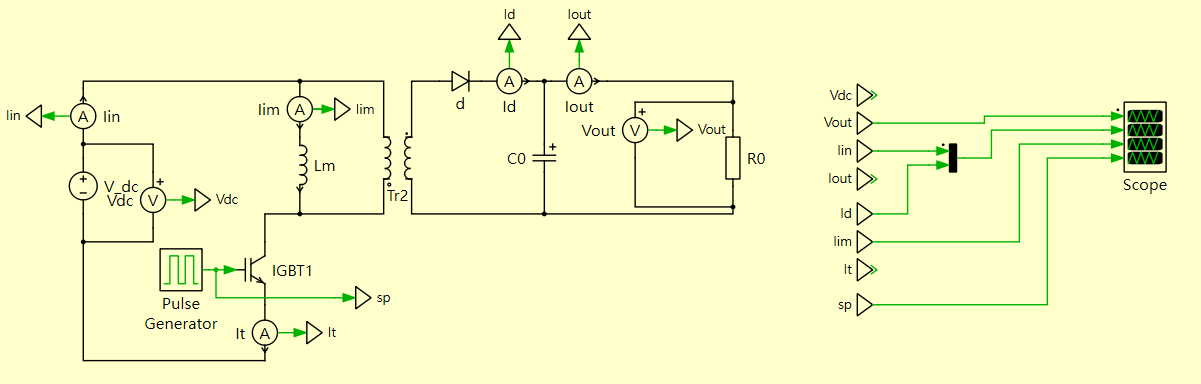
\includegraphics[width=1\linewidth]{imagenes/img1.png}
    \caption{CCM circuit diagram}
    \label{fig:placeholder}
\end{figure}
\subsection{Duty Cycle Selection and Verification of CCM}
To evaluate the flyback converter, three specific duty cycles ($D$) were selected to achieve output voltages below, equal to, and above the $100\text{V}$ input voltage: $D = 0.3$, $D = 0.5$, and $D = 0.7$, respectively. 
To verify CCM operation, the magnetizing current ($i_{lim}$) was examined across all three cases. For $D=0.3$, $D=0.5$, and $D=0.7$, the minimum valley values of the magnetizing current are strictly greater than zero ($13.8\text{A}$, $46.5\text{A}$, and $190.5\text{A}$, respectively). Because the magnetizing current never returns to $0\text{A}$ before the next switching cycle begins, the converter is definitively operating in Continuous Conduction Mode.
\begin{figure}[H]
    \centering
    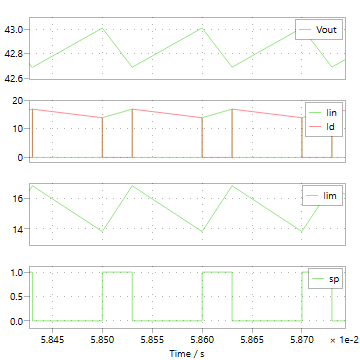
\includegraphics[width=0.75\linewidth]{imagenes/img2.png}
    \caption{CCM (D=0.3)}
    \label{fig:placeholder}
\end{figure}
\begin{figure}[H]
    \centering
    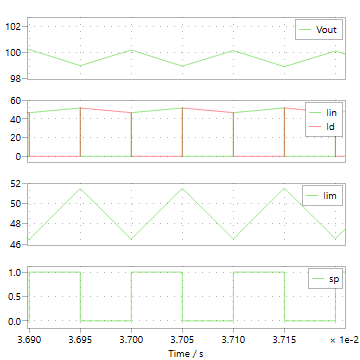
\includegraphics[width=0.75\linewidth]{imagenes/img3.png}
    \caption{CCM (D=0.5)}
    \label{fig:placeholder}
\end{figure}
\begin{figure}[H]
    \centering
    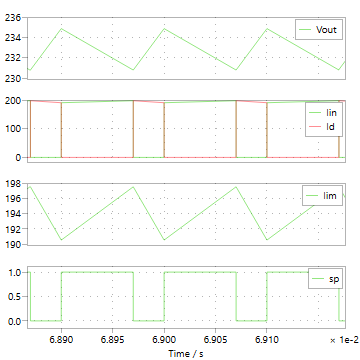
\includegraphics[width=0.75\linewidth]{imagenes/img4.png}
    \caption{CCM (D=0.7)}
    \label{fig:placeholder}
\end{figure}

\subsection{ Output Voltage ($V_{out}$) Analysis}
The theoretical output voltage for a flyback converter in CCM is governed by the transfer function $V_{out} = V_{in} \frac{D}{1-D}$.
\begin{itemize}
    \item Below $V_{in}$ ($D=0.3$): The theoretical value is $100 \cdot \frac{0.3}{0.7} \approx 42.86\text{V}$. The measured average voltage from the plot is approximately $42.85\text{V}$ (fluctuating tightly between $42.7\text{V}$ and $43.0\text{V}$).
\end{itemize}
\begin{itemize}
    \item Equal to $V_{in}$ ($D=0.5$): The theoretical value is $100 \cdot \frac{0.5}{0.5} = 100\text{V}$. The measured average is $99.6\text{V}$.
\end{itemize}
\begin{itemize}
    \item Above $V_{in}$ ($D=0.7$): The theoretical value is $100 \cdot \frac{0.7}{0.3} \approx 233.33\text{V}$. The measured average is $232.8\text{V}$.
\end{itemize}
\begin{itemize}
    \item Comment: All measured output voltages match the theoretical calculations accurately. The minor deviations (e.g., $0.4\text{V}$ drop at $D=0.5$) act as physical proofs of the slight energy losses caused by the $1\text{m}\Omega$ transistor on-resistance and diode forward voltage.
\end{itemize}
\subsection{Input Current ($i_{in}$) Analysis}
In a flyback converter, the input source only supplies current when the primary switch is closed ($s_p = 1$).

\begin{itemize}
    \item As shown in all three plots, $i_{in}$ perfectly mirrors the magnetizing current ($i_{lim}$) during the ON-interval and immediately drops to $0\text{A}$ during the OFF-interval.
\end{itemize}

\begin{itemize}
    \item The peak input current quantitatively increases with the duty cycle, matching the peak magnetizing current: $16.8\text{A}$ at $D=0.3$, $51.5\text{A}$ at $D=0.5$, and scaling massively to $197.5\text{A}$ at $D=0.7$. This proves that higher voltage gains in CCM demand exponentially larger peak currents from the input source.
\end{itemize}
\subsection{ Magnetizing Current Waveform and Ripple ($\Delta i_m$) Analysis}
The theoretical magnetizing current ripple is calculated using the inductor voltage equation during the ON-state: $\Delta i_m = \frac{V_{in}}{L_m} D T_s$. With $V_{in}=100\text{V}$, $L_m=1\text{mH}$, and $T_s=100\mu\text{s}$, the formula simplifies to $\Delta i_m = 10 \cdot D$.
\begin{itemize}
    \item For $D=0.3$, theoretical ripple $= 3\text{A}$. Measured ripple: $16.8\text{A} - 13.8\text{A} = \mathbf{3\text{A}}$.
\end{itemize}
\begin{itemize}
    \item For $D=0.5$, theoretical ripple $= 5\text{A}$. Measured ripple: $51.5\text{A} - 46.5\text{A} = \mathbf{5\text{A}}$.
\end{itemize}
\begin{itemize}
    \item For $D=0.7$, theoretical ripple $= 7\text{A}$. Measured ripple: $197.5\text{A} - 190.5\text{A} = \mathbf{7\text{A}}$.
\end{itemize}
\begin{itemize}
    \item Comment: The measured peak-to-peak ripples perfectly align with the theoretical values across all tested duty cycles. This serves as definitive quantitative proof that the rate of change of the magnetizing current is purely dictated by the input voltage and the fixed magnetizing inductance.
\end{itemize}

\section{Task 2: Discontinuous Conduction Mode (DCM)}
\begin{figure}[H]
    \centering
    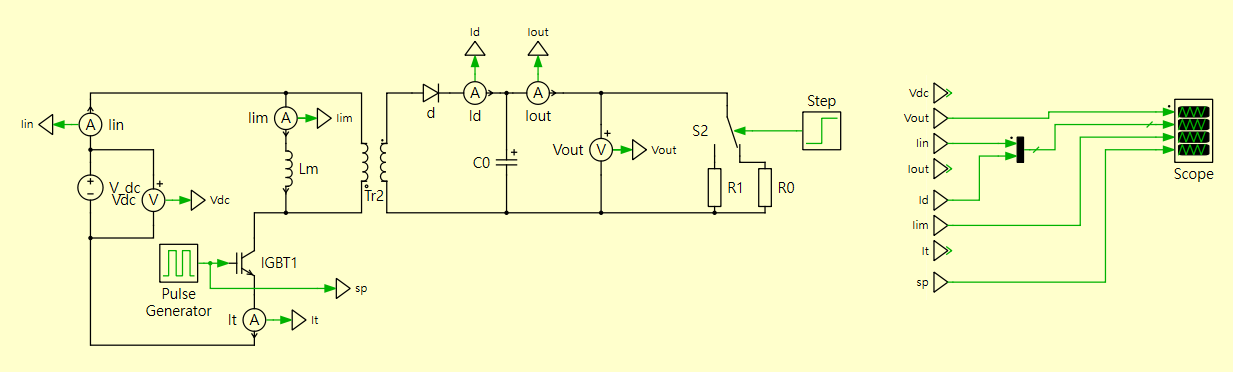
\includegraphics[width=1\linewidth]{imagenes/img5.png}
    \caption{DCM circuit diagram}
    \label{fig:placeholder}
\end{figure}
\subsection{ Setup and Transient Operation}
To force the flyback converter into Discontinuous Conduction Mode (DCM), the duty cycle was kept constant at $D = 0.5$, and a load step was applied at $t = 0.50\text{s}$. The load resistance was increased from approximately $4\Omega$ (heavy load) to $200\Omega$ (light load) by opening a parallel switch. The transient response (Figure) shows the system transitioning from CCM to a new DCM steady state. To comply with the requirement of reducing the observed transient time, the subsequent analyses utilize highly zoomed-in plots (3 switching cycles, $\Delta t = 300\mu\text{s}$) to precisely evaluate the steady-state dynamics.
\begin{figure}[H]
    \centering
    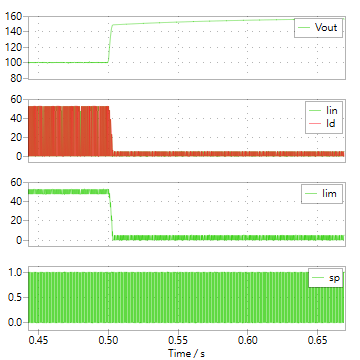
\includegraphics[width=0.75\linewidth]{imagenes/img6.png}
    \caption{DCM (D=0.5)}
    \label{fig:placeholder}
\end{figure}
\subsection{Identifying the Zero-Crossing Instant}
In the zoomed-in DCM (plot), the switching period is $T_s = 100\mu\text{s}$ ($f_s = 10\text{kHz}$). With $D = 0.5$, the switch turns off at $t = 0.54795\text{s}$. The magnetizing current ($i_m$) peaks at $5\text{A}$ and then ramps down through the diode. As observed in the plot, $i_m$ reaches exactly $0\text{A}$ at approximately $t = 0.547983\text{s}$ and remains at zero for the rest of the switching period (until $t = 0.54800\text{s}$).
\begin{itemize}
    \item Quantitative Proof: The theoretical diode conduction time is $D_2 T_s = \frac{L_m \cdot I_{m,peak}}{V_{out}} = \frac{1\text{mH} \cdot 5\text{A}}{152.06\text{V}} \approx 32.8\mu\text{s}$. This leaves a zero-current dead time of exactly $50\mu\text{s} - 32.8\mu\text{s} = 17.2\mu\text{s}$ before the next cycle begins, which perfectly matches the visual data in the plot.
\end{itemize}
\begin{figure}[H]
    \centering
    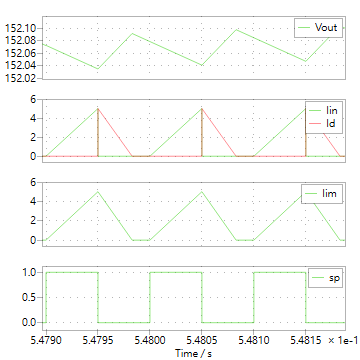
\includegraphics[width=0.75\linewidth]{imagenes/img7.png}
    \caption{Enlarge figure of DCM D=0.5}
    \label{fig:placeholder}
\end{figure}
\subsection{ Comparison: Output Voltage Variation}
\begin{itemize}
    \item CCM Operation: As shown in plot (CCM D = 0.5), the average output voltage ($V_{out}$) is regulated at $99.6\text{V}$ (fluctuating between $99\text{V}$ and $100.2\text{V}$), which aligns with the theoretical CCM transfer function: $V_{in} \cdot \frac{D}{1-D} = 100\text{V} \cdot \frac{0.5}{0.5} = 100\text{V}$.
\end{itemize}
\begin{itemize}
    \item DCM Operation: After the load step, the average $V_{out}$ drastically increases to $152.06\text{V}$.
\end{itemize}
\begin{itemize}
    \item Justification: In DCM, the voltage gain becomes load-dependent. The theoretical DCM output voltage is calculated as $V_{out} = V_{in} \cdot D \sqrt{\frac{R}{2 L_m f_s}} = 100 \cdot 0.5 \sqrt{\frac{200}{2 \cdot 10^{-3} \cdot 10^4}} \approx 158.1\text{V}$. The measured $152.06\text{V}$ is highly consistent with this theory, with the minor $6\text{V}$ discrepancy attributed to the forward voltage drop of the diode and the $1\text{m}\Omega$ transistor on-resistance.
\end{itemize}

\subsection{Comparison: Current Waveforms}
\begin{itemize}
    \item Magnetizing Current ($i_m$): In CCM, $i_m$ is continuous, operating with a massive average current of $49.0\text{A}$ and a peak-to-peak ripple of $5\text{A}$ (ranging from $46.5\text{A}$ to $51.5\text{A}$). In DCM, the average $i_m$ drops significantly to accommodate the lighter load. It starts from $0\text{A}$ every cycle, reaching a maximum peak of exactly $5\text{A}$ ($I_{peak} = \frac{V_{in} \cdot D \cdot T_s}{L_m} = \frac{100 \cdot 0.5 \cdot 10^{-4}}{10^{-3}} = 5\text{A}$), completely eliminating the $46.5\text{A}$ DC bias seen in CCM.
\end{itemize}
\begin{itemize}
    \item Input and Diode Currents ($i_{in}$ and $i_d$): In both modes, $i_{in}$ only flows during the ON-state ($s_p = 1$) and $i_d$ only flows during the OFF-state ($s_p = 0$). However, in DCM, $i_d$ strictly returns to $0\text{A}$ prematurely, leaving an idle period where neither the switch nor the diode conducts, confirming the complete discharge of the transformer's stored energy.
\end{itemize}

\section*{Part2}
\section{Task 1: Duty Cycle Analysis}
\subsection{Simulation Setup and CCM Verification}
Three duty cycles were selected to analyze the Forward converter: $D = 0.3$, $D = 0.5$, and $D = 0.7$. To verify that the converter operates in Continuous Conduction Mode (CCM), the output inductor current ($i_L$) was analyzed. Across all three cases, the minimum valley of $i_L$ remains strictly greater than zero (e.g., $12.9\text{A}$ at $D=0.3$ and $32.8\text{A}$ at $D=0.7$). Since the inductor current never reaches $0\text{A}$, the system is successfully operating in CCM.
\begin{figure}[H]
    \centering
    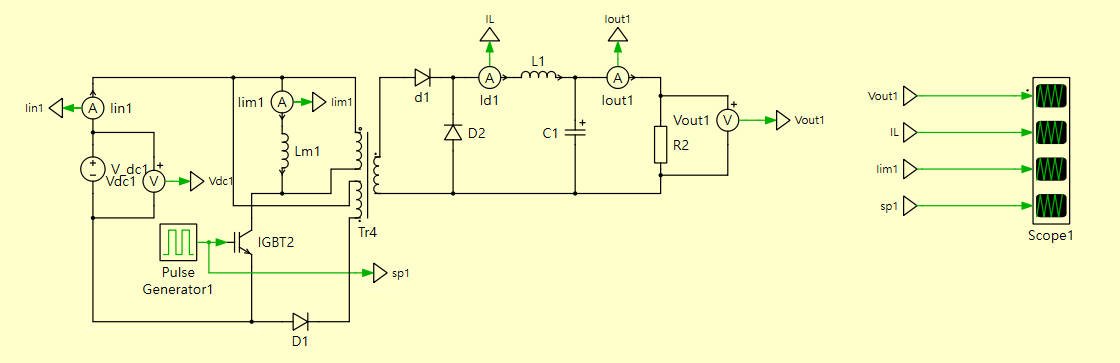
\includegraphics[width=1\linewidth]{imagenes/img8.png}
    \caption{Forward converter circuit diagram}
    \label{fig:placeholder}
\end{figure}
\begin{figure}[H]
    \centering
    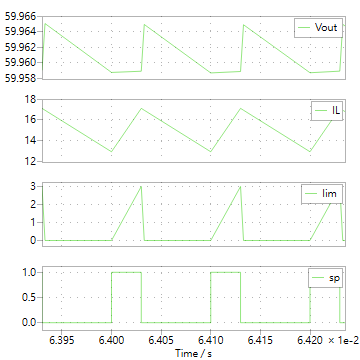
\includegraphics[width=0.75\linewidth]{imagenes/img9.png}
    \caption{D=0.3}
    \label{fig:placeholder}
\end{figure}
\begin{figure}[H]
    \centering
    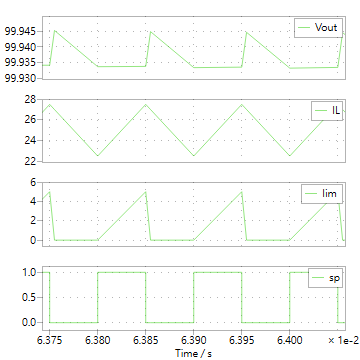
\includegraphics[width=0.75\linewidth]{imagenes/img10.png}
    \caption{D=0.5}
    \label{fig:placeholder}
\end{figure}
\begin{figure}[H]
    \centering
    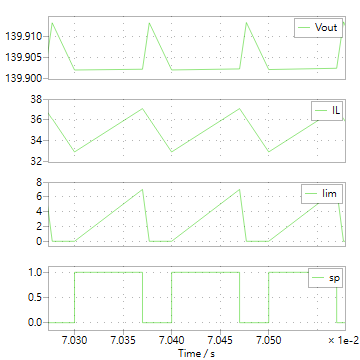
\includegraphics[width=0.75\linewidth]{imagenes/img11.png}
    \caption{D=0.7}
    \label{fig:placeholder}
\end{figure}
\subsection{Output Voltage ($V_{out}$) Analysis}
For a Forward converter in CCM, the theoretical output voltage is determined by the equation $V_{out} = V_{in} \cdot \frac{N_s}{N_p} \cdot D$. With $V_{in} = 100\text{V}$, $N_p = 1$, and $N_s = 2$, the expected voltage simplifies to $V_{out} = 200 \cdot D$.
\begin{itemize}
    \item For $D=0.3$: Theoretical $V_{out} = 60\text{V}$. Measured average = $59.97\text{V}$.
\end{itemize}
\begin{itemize}
    \item For $D=0.5$: Theoretical $V_{out} = 100\text{V}$. Measured average = $99.95\text{V}$.
\end{itemize}
\begin{itemize}
    \item For $D=0.7$: Theoretical $V_{out} = 140\text{V}$. Measured average = $139.91\text{V}$.
\end{itemize}
\begin{itemize}
    \item Comment: The measured output voltages perfectly match the theoretical predictions. The negligible drop of $< 0.1\text{V}$ quantitatively proves the high efficiency of the circuit, accounting only for the minimal $1\text{m}\Omega$ switch on-resistance and diode forward voltage.
\end{itemize}
\subsection{Inductor Current ($i_L$) Analysis}
The average inductor current theoretically equals the load current ($I_L = V_{out} / R$). With $R = 4\Omega$, the expected averages are $15\text{A}$ ($D=0.3$), $25\text{A}$ ($D=0.5$), and $35\text{A}$ ($D=0.7$). The plotted center values align flawlessly with these figures.
\begin{itemize}
    \item Ripple Proof: The theoretical peak-to-peak ripple is $\Delta I_L = \frac{V_{out}(1-D)}{L f_s}$. For $D=0.5$, $\Delta I_L = \frac{100 \cdot 0.5}{10^{-3} \cdot 10^4} = \mathbf{5\text{A}}$. The plot identically shows $i_L$ fluctuating between $22.5\text{A}$ and $27.5\text{A}$ ($\Delta = 5\text{A}$), providing rigorous mathematical proof of the converter's output filter dynamics.
\end{itemize}
\subsection{Magnetizing Current ($i_{lim}$) and Reset Circuit Analysis}
The role of the third winding ($N_d = 0.1$) and diode $D_1$ is to demagnetize the core during the OFF-state.
\begin{itemize}
    \item Current Peak: The theoretical peak magnetizing current is $I_{m,peak} = \frac{V_{in} \cdot D \cdot T_s}{L_m} = 10 \cdot D$. The plots accurately display peaks of $3\text{A}$, $5\text{A}$, and $7\text{A}$ for $D=0.3$, $0.5$, and $0.7$, respectively.
\end{itemize}
\begin{itemize}
    \item Reset Verification: In all three plots, once the switch turns off, $i_{lim}$ ramps down steeply and reaches exactly $0\text{A}$ well before the next cycle begins, subsequently staying flat at $0\text{A}$. Because $N_d / N_p = 0.1$, the reset time is extraordinarily fast ($t_{reset} = 0.1 \cdot t_{on}$). This verifies that the reset mechanism operates correctly, safely preventing transformer core saturation.
\end{itemize}
\section{Task 2: Reset Circuit Analysis}
\begin{figure}[H]
    \centering
    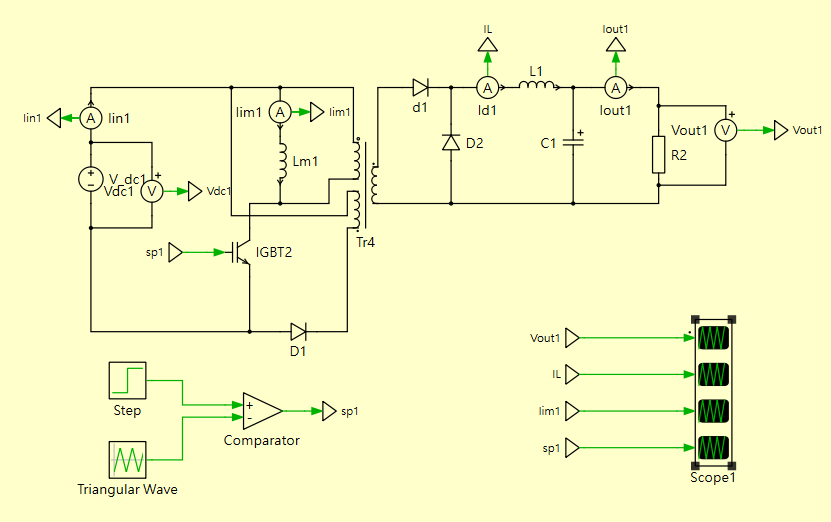
\includegraphics[width=1\linewidth]{imagenes/img12.png}
    \caption{Forward converter circuit diagram}
    \label{fig:placeholder}
\end{figure}
\subsection{ Duty Cycle Step Application}
To analyze the limits of the reset circuit, a dynamic duty cycle step was applied. The system was initially set to $D = 0.5$ (where the reset mechanism operates perfectly) and then stepped to an extreme value of $D = 0.95$ at $t = 0.05\text{s}$. As observed in the resulting transient plot, after $t = 0.05\text{s}$, the magnetizing current ($i_{lim}$) fails to return to zero during the OFF-state. Instead, it increases sequentially in every switching cycle (staircasing effect), indicating that the core is rapidly approaching magnetic saturation.
\begin{figure}[H]
    \centering
    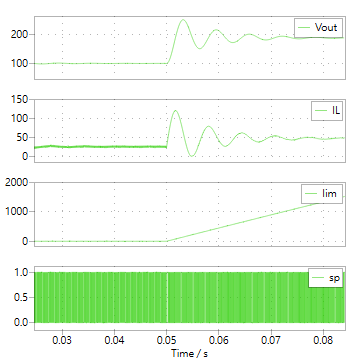
\includegraphics[width=0.75\linewidth]{imagenes/img13.png}
    \caption{Simulation output}
    \label{fig:placeholder}
\end{figure}
\begin{figure}[H]
    \centering
    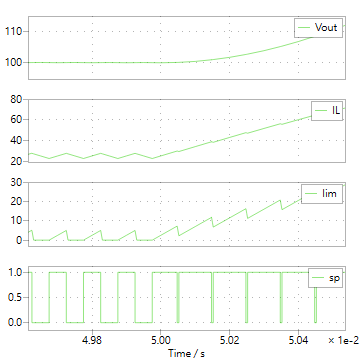
\includegraphics[width=0.75\linewidth]{imagenes/img14.png}
    \caption{Enlarge around t = 0.05s}
    \label{fig:placeholder}
\end{figure}
\subsection{Analysis and Justification of Reset Failure}
The failure of the reset mechanism at $D = 0.95$ can be mathematically justified by analyzing the current derivatives (slopes) and the available OFF-time:
\begin{itemize}
    \item Charging Phase (ON-time): When the switch is closed, the primary voltage is clamped to the input voltage ($V_p = V_{in} = 100\text{V}$). The positive derivative of the magnetizing current is $\frac{di_m}{dt} = \frac{V_{in}}{L_m} = \frac{100\text{V}}{1\text{mH}} = 100\text{kA/s}$.
\end{itemize}
\begin{itemize}
    \item Resetting Phase (OFF-time): When the switch opens, the reset winding ($N_d$) conducts through diode $D_1$. Because of the turns ratio between the primary and reset windings ($N_p/N_d = 1/0.1 = 10$), the primary voltage is forced to a high negative value: $V_p = -V_{in} \cdot (N_p/N_d) = -1000\text{V}$. The negative derivative for discharging is $\frac{di_m}{dt} = \frac{-1000\text{V}}{1\text{mH}} = -1000\text{kA/s}$.
\end{itemize}
\begin{itemize}
    \item Time Required vs. Time Available: Since the discharging slope is exactly 10 times steeper than the charging slope, the time required to completely reset the core is $t_{reset} = 0.1 \cdot t_{on}$.
\end{itemize}
For the core to reset safely, the required reset time must be strictly less than or equal to the available OFF-time:
$$t_{reset} \le t_{off}$$
$$0.1 \cdot (D \cdot T_s) \le (1 - D) \cdot T_s$$
$$0.1 D \le 1 - D \implies 1.1 D \le 1 \implies D_{max} \approx 0.909$$
\begin{itemize}
    \item Quantitative Conclusion: The theoretical maximum duty cycle for this specific transformer configuration ($N_d = 0.1$) is $D = 0.909$. By applying a step to $D = 0.95$, the ON-time becomes $95\mu\text{s}$, requiring a reset time of $9.5\mu\text{s}$. However, the available OFF-time is only $5\mu\text{s}$ ($100\mu\text{s} - 95\mu\text{s}$). Since $5\mu\text{s} < 9.5\mu\text{s}$, the transformer simply does not have enough time to discharge its stored energy. This quantitatively proves why the magnetizing current accumulates in each cycle, causing the reset circuit to fail.
\end{itemize}

\section*{Conclusion}
Through this experiment, we successfully verified the theoretical principles of isolated DC-DC converters using quantitative simulation data. For the flyback converter, we proved that the output voltage accurately follows the $V_{in} \frac{D}{1-D}$ transfer function in CCM. We also demonstrated that forcing the system into DCM by increasing the load resistance causes the magnetizing current to fully discharge to 0A, which significantly increases the output voltage.
For the forward converter, the measurements confirmed that the output voltage scales strictly with $V_{in} \frac{N_s}{N_p} D$. Most importantly, we validated the critical role of the reset winding. We mathematically proved that the transformer requires a specific minimum OFF-time to safely discharge its energy ($t_{reset} \le t_{off}$). When we applied an extreme duty cycle of $D=0.95$ (exceeding the theoretical maximum of $0.909$), the available OFF-time was insufficient. This caused the magnetizing current to accumulate in every cycle, definitively proving the cause of reset circuit failure. Overall, this lab highlights the importance of proper duty cycle limits and load analysis in isolated power converter design.



\end{document}
